\section{Experimental results}

\subsection{Simple function task}

Our simple function task samples an input vector $\mathbf{x}$ from a uniform distribution. From this input vector, the sum of two subsets $a$ and $b$ are then computed. Finally the target $t$ is then an operation performed on $a$ and $b$ (e.g. $a \cdot b$). This is identical to the task by the same name in the Original NALU paper \cite{trask-nalu}. Except that we parameterize it in order to compare the models for different configurations, see figure \ref{fig:simple-function-task-problem}. To make comparison simple, we define a set of default parameters (table \ref{tab:simple-function-task-defaults}) and only vary one of them at the time.

\begin{figure}[H]
\centering
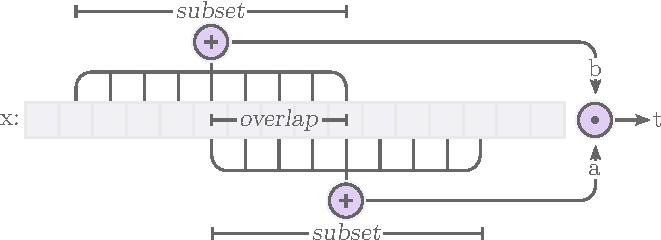
\includegraphics[scale=0.8]{graphics/function_task_static_problem.pdf}
\caption{Dataset is parameterized into ``Input Size'', ``Subset Ratio'', ``Overlap Ratio'', an Operation (here showing multiplication), ``Interpolation Range'' and ``Extrapolation Range'' from which the data set sampled.}
\label{fig:simple-function-task-problem}
\end{figure}

\begin{table}[H]
\caption{Default dataset parameters}
\label{tab:simple-function-task-defaults}
\centering
\begin{tabular}{r l}
\toprule
 Parameter Name & Default Value \\
 \midrule
 Input Size & 100 \\
 Subset Ratio & 0.25 \\
 Overlap Ratio & 0.5 \\
 Interpolation Range & $U[1,2]$ \\
 Extrapolation Range & $U[1,6]$ \\
 \bottomrule
\end{tabular}
\end{table}

Normally one would report the interpolation and extrapolation loss. However, the complex approximations that one would typically see in neural networks are not considered good enough. The goal is to achieve a solution that is sufficiently close to a perfect solution. Because there can be many valid permutations of a perfect solution, especially for addition, a solution is judged firsts on the final extrapolation error, and then on a sparsity error.

All errors; extrapolation, interpolation, and sparsity are computed every 1000 iterations for 2048 new observations. Because the interpolation and extrapolation errors are quite noisy, even for a near perfect solution. The median over the last 100 measurements is reported.

A model is considered a success if the extrapolation median is less than $\epsilon = 0.2$. This value was acquired by inspecting the error of a near perfect solution. \todo{Get a better critation.}

The sparsity error is computed as in equation \ref{eq:sparsity-error}, and is only considered for the models that did solve the last.
\begin{equation}
E_\mathrm{sparsity} = \max_{h_{\ell-1}, h_{\ell}} \min(|W_{h_{\ell-1},h_\ell}|, |1 - |W_{h_{\ell-1},h_\ell}||)
\label{eq:sparsity-error}
\end{equation}

The first iteration for which $\mathrm{extrapolation} < \epsilon$, is also reported. Again, only models that did solve the task are considered.

\begin{figure}[H]
\centering
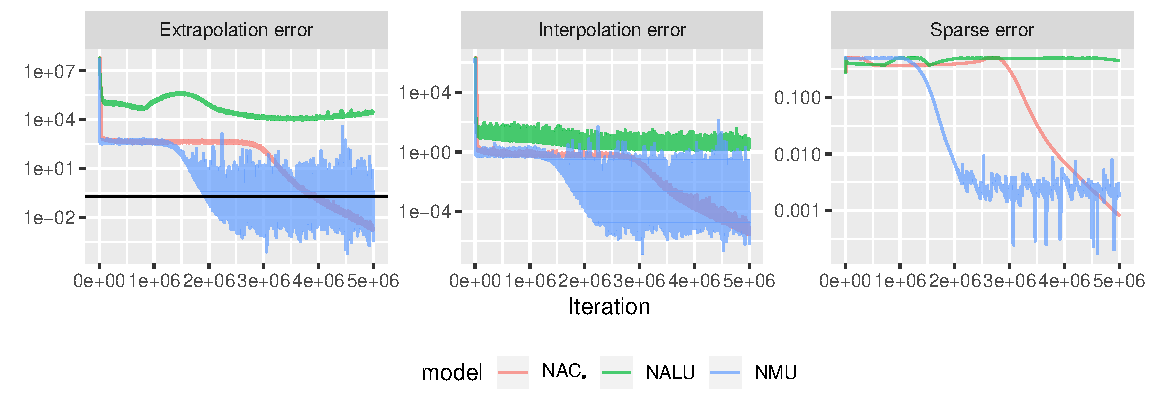
\includegraphics[width=\linewidth]{paper/results/function-task-static-example.pdf}
\caption{Example of exploration error, interpolation error, and sparsity error, for the task $a \cdot b$ with the default dataset parameters.}
\end{figure}

\subsubsection{Very simple function}

To empirically validate the theoretical problems with $\mathrm{NAC}_{\bullet}$, let's consider the very simple problem shown earlier in figure \ref{fig:nac-mul-eps-issue}. That is $x \in \mathbb{R}^4$, $a = x_1 + x_2$ and $b = x_1 + x_2 + x_3 + x_4$. The solution to this problem is that seen in equation \ref{eq:very-simple-function-ideal-solution}.
\begin{equation}
    \mathbf{W}_1 = \begin{bmatrix}
    1 & 1 & 0 & 0 \\
    1 & 1 & 1 & 1
    \end{bmatrix}, \mathbf{W}_2 = \begin{bmatrix}
    1 & 1
    \end{bmatrix}
    \label{eq:very-simple-function-ideal-solution}
\end{equation}

Each model is trained 100 times with different seeds, and stopped after 200000 iterations. Default Adam optimization is used, with a mini-batch size of 128 observations. The results (as seen in table \ref{tab:very-simple-function-results}), shows that NMU have a much higher success rate and converges much faster. The few cases that did not converge successfully are because of underflow when $w = 0$ in the NMU layer.

\begin{table}[!h]

\caption{\label{tab:very-simple-function-results}Shows the success-rate, at what global step the model converged at, and the sparsity error for all weight matrices, with 95\% confidence interval. Best result is highlighed.}
\centering
\begin{tabular}{crllll}
\toprule
\multicolumn{1}{c}{Op} & \multicolumn{1}{c}{Model} & \multicolumn{1}{c}{Success} & \multicolumn{2}{c}{Solved at} & \multicolumn{1}{c}{Sparsity error} \\
\cmidrule(l{3pt}r{3pt}){1-1} \cmidrule(l{3pt}r{3pt}){2-2} \cmidrule(l{3pt}r{3pt}){3-3} \cmidrule(l{3pt}r{3pt}){4-5} \cmidrule(l{3pt}r{3pt}){6-6}
 &  & Rate & Median & Mean & Mean\\
\midrule
 & $\mathrm{NAC}_{\bullet}$ & $13\% {~}^{+8\%}_{-5\%}$ & $5.5 \cdot 10^{4}$ & $5.9 \cdot 10^{4} {~}^{+7.8 \cdot 10^{3}}_{-6.6 \cdot 10^{3}}$ & $7.5 \cdot 10^{-6} {~}^{+2.0 \cdot 10^{-6}}_{-2.0 \cdot 10^{-6}}$\\

 & NALU & $26\% {~}^{+9\%}_{-8\%}$ & $7.0 \cdot 10^{4}$ & $7.8 \cdot 10^{4} {~}^{+6.2 \cdot 10^{3}}_{-8.6 \cdot 10^{3}}$ & $9.2 \cdot 10^{-6} {~}^{+1.7 \cdot 10^{-6}}_{-1.7 \cdot 10^{-6}}$\\

\multirow{-3}{*}{\centering\arraybackslash $\bm{\times}$} & NMU & $\mathbf{94\%} {~}^{+3\%}_{-6\%}$ & $\mathbf{1.4 \cdot 10^{4}}$ & $\mathbf{1.4 \cdot 10^{4}} {~}^{+2.2 \cdot 10^{2}}_{-2.1 \cdot 10^{2}}$ & $\mathbf{2.6 \cdot 10^{-8}} {~}^{+6.4 \cdot 10^{-9}}_{-6.4 \cdot 10^{-9}}$\\
\bottomrule
\end{tabular}
\end{table}


\subsubsection{Defaults}

To compare on the exact same task as used in the Original NALU paper \cite{trask-nalu}. We report the success rate, the iteration which the model converged, and the sparsity error in table \ref{tab:function-task-static-defaults}. The models are trainined for 5000000 iterations. Default Adam optimization is used, with a mini-batch size of 128 observations. The NMU model is an NAU layer followed by an NMU layer. Likewise the  $\mathrm{NAC}_{\bullet}$ model, is a $\mathrm{NAC}_{+}$ layer followed by a $\mathrm{NAC}_{\bullet}$ layer.

As seen the NMU model, unlike the $\mathrm{NAC}_{\bullet}$ model always converges, and even when $\mathrm{NAC}_{\bullet}$ model converges the NMU models converges about twice as fast.

The NAU model, like the $\mathrm{NAC}_{+}$ model, always converges. However, NAU model converges more than twice as fast. It even converges faster than a Linear model. Also notice that the $\mathrm{NAC}_{+}$ model have a poor sparsity error. This is because it doesn't bias to $\{-1, 0, -1\}$.

\begin{table}[!h]

\caption{\label{tab:function-task-static-defaults}Shows the success-rate for $\mathcal{L}_{\mathbf{W}_1, \mathbf{W}_2} < \mathcal{L}_{\mathbf{W}_1^\epsilon, \mathbf{W}_2^*}$, at what global step the model converged at, and the sparsity error for all weight matrices.}
\centering
\begin{tabular}{crllll}
\toprule
\multicolumn{1}{c}{Op} & \multicolumn{1}{c}{Model} & \multicolumn{1}{c}{Success} & \multicolumn{2}{c}{Solved at} & \multicolumn{1}{c}{Sparsity error} \\
\cmidrule(l{3pt}r{3pt}){1-1} \cmidrule(l{3pt}r{3pt}){2-2} \cmidrule(l{3pt}r{3pt}){3-3} \cmidrule(l{3pt}r{3pt}){4-5} \cmidrule(l{3pt}r{3pt}){6-6}
 &  & Rate & Median & Mean & Mean\\
\midrule
 & $\mathrm{NAC}_{\bullet}$ & $30\%$ & $2.5 \cdot 10^{6}$ & $2.5 \cdot 10^{6} \pm 1.5 \cdot 10^{6}$ & $\mathbf{3.9 \cdot 10^{-4} \pm 9.4 \cdot 10^{-4}}$\\

 & Linear & $0\%$ & --- & --- & ---\\

 & NALU & $0\%$ & --- & --- & ---\\

\multirow{-4}{*}{\centering\arraybackslash $\bm{\times}$} & NMU & $\mathbf{90\%}$ & $\mathbf{1.4 \cdot 10^{6}}$ & $\mathbf{1.6 \cdot 10^{6} \pm 5.6 \cdot 10^{5}}$ & $1.8 \cdot 10^{-3} \pm 1.1 \cdot 10^{-3}$\\
\cmidrule{1-6}
 & $\mathrm{NAC}_{+}$ & $\mathbf{100\%}$ & $6.0 \cdot 10^{4}$ & $7.1 \cdot 10^{4} \pm 2.4 \cdot 10^{4}$ & $4.8 \cdot 10^{-1} \pm 2.0 \cdot 10^{-2}$\\

 & Linear & $\mathbf{100\%}$ & $4.2 \cdot 10^{4}$ & $\mathbf{4.2 \cdot 10^{4} \pm 1.9 \cdot 10^{3}}$ & $6.1 \cdot 10^{-1} \pm 1.2 \cdot 10^{-1}$\\

 & NALU & $0\%$ & --- & --- & ---\\

\multirow{-4}{*}{\centering\arraybackslash $\bm{+}$} & NAU & $\mathbf{100\%}$ & $\mathbf{1.8 \cdot 10^{4}}$ & $7.0 \cdot 10^{5} \pm 9.2 \cdot 10^{5}$ & $\mathbf{1.7 \cdot 10^{-3} \pm 8.0 \cdot 10^{-4}}$\\
\cmidrule{1-6}
 & $\mathrm{NAC}_{+}$ & $\mathbf{100\%}$ & $8.0 \cdot 10^{3}$ & $1.5 \cdot 10^{6} \pm 1.5 \cdot 10^{6}$ & $4.6 \cdot 10^{-1} \pm 2.9 \cdot 10^{-2}$\\

 & Linear & $\mathbf{100\%}$ & $1.1 \cdot 10^{6}$ & $1.9 \cdot 10^{6} \pm 1.3 \cdot 10^{6}$ & $3.7 \cdot 10^{-1} \pm 1.1 \cdot 10^{-1}$\\

 & NALU & $20\%$ & $3.6 \cdot 10^{6}$ & $3.6 \cdot 10^{6} \pm 1.3 \cdot 10^{7}$ & $4.7 \cdot 10^{-1} \pm 3.3 \cdot 10^{-1}$\\

\multirow{-4}{*}{\centering\arraybackslash $\bm{-}$} & NAU & $\mathbf{100\%}$ & $\mathbf{4.0 \cdot 10^{3}}$ & $\mathbf{4.2 \cdot 10^{3} \pm 3.0 \cdot 10^{2}}$ & $\mathbf{1.9 \cdot 10^{-3} \pm 4.2 \cdot 10^{-4}}$\\
\bottomrule
\end{tabular}
\end{table}


\subsubsection{Exploration of dataset parameters}

Finally, the parameters from which the dataset is constructed are considered for just the multiplication problem ($a \cdot b$). The setup is the same the results from table \ref{tab:function-task-static-defaults}. The results are visualized in in figure \ref{fig:simple-fnction-static-input-size}, \ref{fig:simple-fnction-static-overlap}, \ref{fig:simple-fnction-static-range}, and \ref{fig:simple-fnction-static-subset}. Errors bars show the upper and lower 10\% quantile, computed over 10 different seeds for each configuration. The center shows the mean of those 10 observations.

Generally the NMU performs far better than both $\mathrm{NAC}_{\bullet}$ and NALU. Some important observations to make:

\begin{itemize}
\item Input size $> 100$. The NMU model's success-rate very suddenly decreases when the input size is greater than 100. We have been unable to explain why this happens. We suspect it is a problem with the signal-to-noie ratio of the problem. However the result is also seen if the mini-batch size is dramatically increased.
\item Overlap ratio $= 0$: Both the NMU and also the $\mathrm{NAC}_{\bullet}$ when it does converge, finds a suboptimal solution where in the addition layer $w=1$ for the overlapping input between $a$ and $b$, and $w = 0$ for where the input isn't used. However when an input-scalar is only used in either $a$ or $b$, convergence the corresponding weights is difficult and slow. Thus the lower the overlap ratio is, the harder the problem is.
\end{itemize}

\begin{figure}[H]
\centering
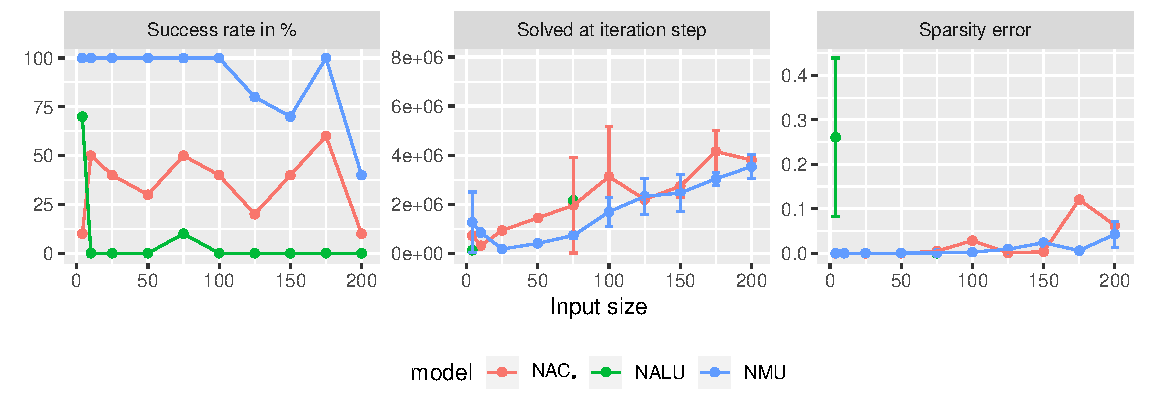
\includegraphics[width=\linewidth]{results/simple_function_static_input_size.pdf}
\caption{Shows the effect of the input size, on the simple function task problem.}
\label{fig:simple-fnction-static-input-size}
\end{figure}

\begin{figure}[h]
\centering
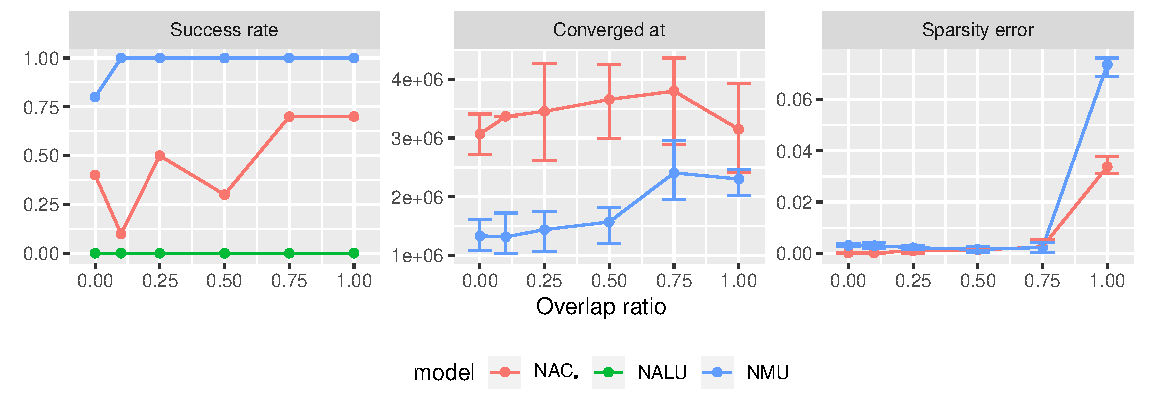
\includegraphics[width=\linewidth]{results/simple_function_static_overlap.pdf}
\caption{Shows the effect of the overlap ratio, on the simple function task problem.}
\label{fig:simple-fnction-static-overlap}
\end{figure}

\begin{figure}[h]
\centering
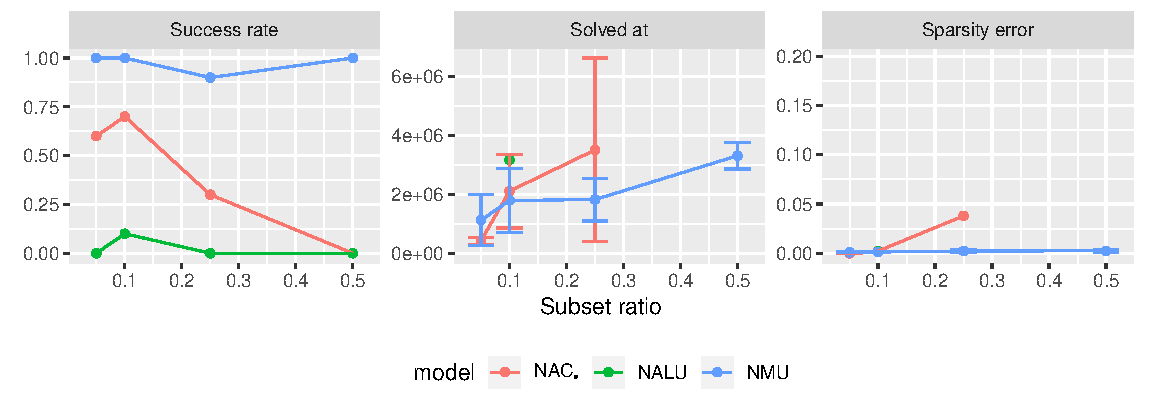
\includegraphics[width=\linewidth]{results/simple_function_static_subset.pdf}
\caption{Shows the effect of the subset ratio, on the simple function task problem.}
\label{fig:simple-fnction-static-subset}
\end{figure}

\begin{figure}[h]
\centering
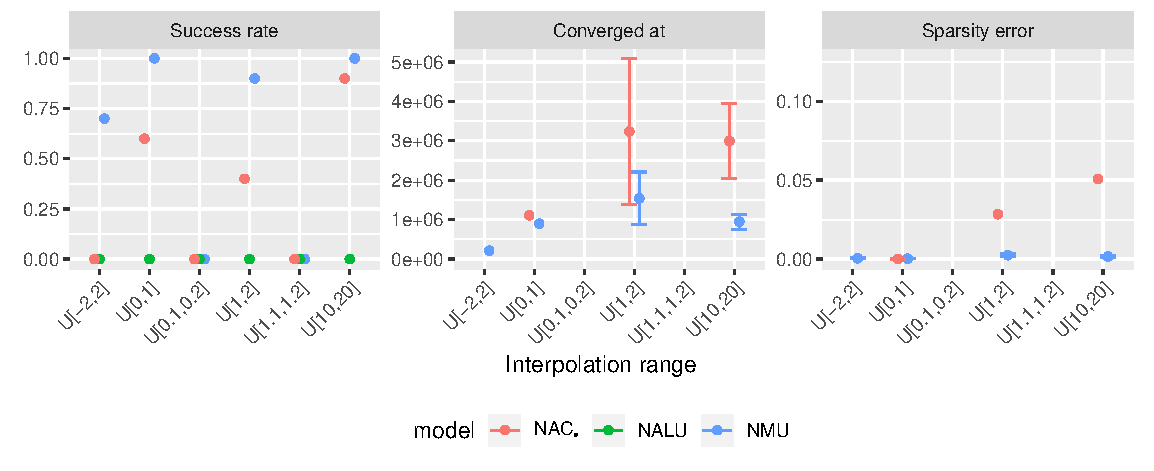
\includegraphics[width=\linewidth]{results/simple_function_static_range.pdf}
\caption{Shows the effect of the interpolation range. For each interpolation range, the following extrapolation ranges are used: ${\mathrm{U}[-2,2] \rightarrow \mathrm{U}[-6,6]}$, ${\mathrm{U}[0,1] \rightarrow \mathrm{U}[0,5]}$, ${\mathrm{U}[0.1,0.2] \rightarrow \mathrm{U}[0,2]}$, ${\mathrm{U}[1,2] \rightarrow \mathrm{U}[1,6]}$, ${\mathrm{U}[10, 20] \rightarrow \mathrm{U}[1, 40]}$.}
\label{fig:simple-fnction-static-range}
\end{figure}

\subsection{Sequential MNIST}

\todo[inline]{Still waiting for results}

\begin{figure}[H]
\centering
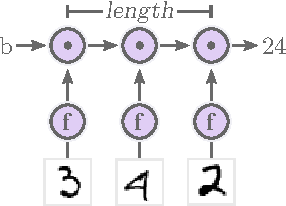
\includegraphics[scale=1]{graphics/mnist_sequence_problem.pdf}
\caption{Lorem Ipsum.}
\end{figure}

